% !TeX TXS-program:compile = txs:///pdflatex/[--shell-escape]
\documentclass[handout, aspectratio=169, 10pt]{beamer}

% packages
\usepackage{newpxmath} % math font is Palatino compatible
% \usepackage[nomath]{fontspec}

\usepackage{setspace}
\usepackage{xcolor}
\usepackage{soul} % for \st
\usepackage{hyperref} % for links
\definecolor{links}{HTML}{2A1B81}
\hypersetup{colorlinks,linkcolor=,urlcolor=links}


% table stuff
\usepackage{chronosys}
\usepackage{verbatim}
% \pagenumbering{arabic}
\usepackage{tabularx}
\usepackage{booktabs}
\usepackage{ragged2e}
\usepackage{mathtools}

% R Code
\usepackage{listings}
\usepackage{courier}
\lstset{basicstyle=\scriptsize\ttfamily,breaklines=true}
\lstset{framextopmargin=50pt,frame=bottomline}

% themes
\usetheme[progressbar=frametitle, block=fill]{metropolis}
\useoutertheme{metropolis}
\useinnertheme{metropolis}

% colors
\definecolor{dimwhite}{rgb}{0.99, 0.99, 0.99}
\definecolor{charcoal}{rgb}{0.21, 0.27, 0.31}
\definecolor{slategray}{rgb}{0.44, 0.5, 0.56}
\definecolor{dimgray}{rgb}{0.41, 0.41, 0.41}
\definecolor{bleudefrance}{rgb}{0.19, 0.55, 0.91}

% beamer options
\setbeamercolor{author}{fg=charcoal}
\setbeamercolor{background canvas}{bg=white}
\setbeamercolor{section in toc}{fg=charcoal}
\setbeamercolor{subsection in toc}{fg=dimgray}
\setbeamercolor{frametitle}{bg=dimwhite, fg=charcoal}
\setbeamercolor{progress bar}{fg=slategray, bg=fg!50!black!30}
\setbeamercovered{transparent}
\setbeamertemplate{itemize items}[triangle]
\setbeamertemplate{itemize subitem}[circle]
\setbeamertemplate{itemize subsubitem}[square]
\setbeamersize{text margin left=7mm,text margin right=7mm} 

% new commands
\newcommand{\q}[1]{``#1''}
\newcommand{\hs}[1]{\textsc{\hfill\scriptsize\color{dimgray}#1}}
\newcommand{\g}[1]{{\color{gray}#1}}
\newcommand{\dg}[1]{{\color{dimgray}#1}}
\newcommand{\sg}[1]{{\color{slategray}#1}}
\newcommand{\bdf}[1]{{\color{bleudefrance}#1}}
\newcommand{\itemcolor}[1]{\renewcommand{\makelabel}[1]{\color{#1}\hfil ##1}}
\newcommand\Wider[2][2em]{
\makebox[\linewidth][c]{
  \begin{minipage}{\dimexpr\textwidth+#1\relax}
  \raggedright#2
  \end{minipage}
  }
}

% misc
\linespread{1.35}

% minted (risky)
\usepackage[cache=false]{minted}

% Math stuff
\newcommand{\norm}[1]{\left\lVert#1\right\rVert}
\newcommand{\R}{\mathbb{R}}
\newcommand{\E}{\mathbb{E}}
\newcommand{\V}{\mathbb{V}}
\newcommand{\probP}{\text{I\kern-0.15em P}}
\newcommand{\ol}{\overline}
%\newcommand{\ul}{\underline}
\newcommand{\pp}{{\prime \prime}}
\newcommand{\ppp}{{\prime \prime \prime}}
\newcommand{\policy}{\gamma}
\newcommand{\plim}{ \overset{p}{\to}}
\newcommand{\hnot}{ \overset{H_0}{\to}}

% Causal Graphs
\usetikzlibrary{shapes,decorations,arrows,calc,arrows.meta,fit,positioning}
\tikzset{
    -Latex,auto,node distance =1 cm and 1 cm,semithick,
    state/.style ={ellipse, draw, minimum width = 0.7 cm},
    point/.style = {circle, draw, inner sep=0.04cm,fill,node contents={}},
    bidirected/.style={Latex-Latex,dashed},
    el/.style = {inner sep=2pt, align=left, sloped}
}
% \documentclass[english,xcolor={dvipsnames},aspectratio=169,10pt]{beamer}
% \usepackage[italic]{mathastext}

% \usepackage{float}`
% \usepackage{amsmath}
% \usepackage{amssymb}
% \usepackage{graphicx}
% \usepackage{setspace}
% \usepackage[outdir=./]{epstopdf}
% \usepackage{listings}

% \usepackage{caption,subcaption}
% \usepackage{booktabs}
% \usepackage[flushleft]{threeparttable}


% \usepackage{hyperref}
% \hypersetup{
%     colorlinks=true,
%     linkcolor=blue,
%     filecolor=magenta,      
%     urlcolor=blue,
% }


%    \lstset{language=R,
%            basicstyle=\ttfamily\scriptsize,
%            keywordstyle=\color{blue}\ttfamily,
%            stringstyle=\color{red}\ttfamily,
%            commentstyle=\color{green}\ttfamily,
%           breaklines=true
%           }


% \usepackage{siunitx}
% \sisetup{
% input-symbols = {()},
% group-digits  = false,
% explicit-sign
% }

% %\usetheme{CambridgeUS}
% \usetheme{Boadilla}
% \usecolortheme{seahorse}

% \setbeamertemplate{itemize subsubitem}{\tiny\raise1.5pt\hbox{\donotcoloroutermaths$\blacktriangleright$}}


% \usepackage{tikz}
% \usepackage{pgfplots}
% \pgfplotsset{compat=1.7}
% \usetikzlibrary{arrows, shapes, snakes, patterns, angles, quotes}

% \makeatletter


% \usepackage{setspace}
% \usepackage[normalem]{ulem}
\setbeamersize{text margin left=10pt,text margin right=10pt}

% \makeatother

% \usepackage{babel}

\begin{document}


\title[L4 - Inference and Standard Errors]{ Econometrics I}
\subtitle{Lecture 4: Inference and Standard Errors}
\author{Chris Conlon}
\date{Fall 2025}
\maketitle


\begin{frame}
\begin{center}
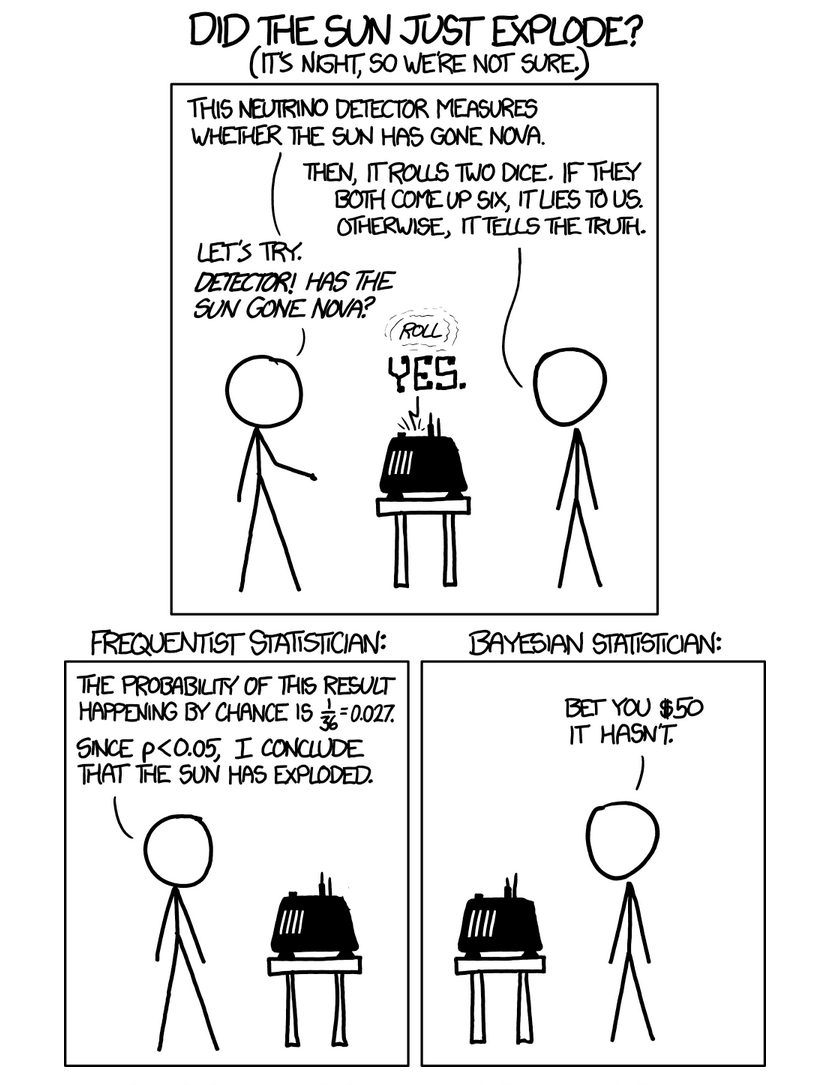
\includegraphics[height=.92\textheight]{explode} \\
{\tiny Source: xkcd.com}
\end{center}
\end{frame}


\begin{frame}{Hypothesis testing}
\begin{itemize}
	\item We are often interested in testing theories, or testing hypotheses about
	the values of certain parameters

	\medskip
	\item Simplest example: testing whether mean of a variable $\mu_x \equiv E\left[X\right]$ 
	is different from a particular value:\[
\begin{array}{c}
H_{0}:\qquad\mu_{x}=a\\
H_{1}:\qquad\mu_{x}\ne a
\end{array}
\]

	\medskip
	\item A hypothesis test typically involves a {\bf null hypothesis} and {\bf alternative hypothesis}. 
	The alternative hypothesis could also be about a particular value ($H_{1}:\mu_{x}= b$, or 
	a one-sided rejection of the null ($H_{1}:\mu_{x}>a$).


\end{itemize}
\end{frame}



\begin{frame}{Review: z test}
\begin{itemize}
	\item If $X_i$ is i.i.d. normal with \emph{known} variance $\sigma^2$, then \[
		\overline{X} \sim \mathcal{N} \left( \mu_x, \sigma^{2}/n \right)
	\]


	\item In this case, we know the distribution of our estimate $\overline{X}$. We can test\[
H_{0}:\mu_{x}=a \qquad H_{1}:\mu_{x}\ne a
\]
using a {\bf z test}.

	\item We construct the test statistic, which under the null hypothesis has the standard normal distribution:
	\begin{align*}		z = \frac{ \overline{X} - a}{n^{-1/2}\sigma}
	 \overset{d}{\to} \mathcal{N} \left( 0,1\right)
	 \end{align*}
\end{itemize}
\end{frame}



\begin{frame}{Level and Size of Test}
\begin{itemize}
	\item The {\bf size} (or {\bf level}) of a test is the probability of rejection if the null hypothesis is true. 
	\emph{The size is the rate of false positives or type I errors.}

	\item When hypothesis testing, we make it hard to reject the null hypothesis. We typically choose the 
	size of the test to be small (most commonly, .01 or .05).

\end{itemize}
\end{frame}




\begin{frame}{Power of Test}
\begin{itemize}

	\item We typically want to reject only for the outcomes that are least likely under the null
	hypothesis (or relatively more likely under the alternative hypothesis than the null). For
	the z test above, we reject only in the tails of the normal distribution. See: Neyman-Pearson Lemma.
	
	\medskip
	\item Choosing the rejection region appropriately maximizes the test's {\bf power}, the 
	probability of rejecting the null hypothesis when it is indeed false. Power is often harder
	to quantify and not something we typically choose. Power is one minus the rate of
	type II errors (\textbf{false negatives}), or failures to reject the null hypothesis when it is false. 
\end{itemize}
\end{frame}



\begin{frame}{Rejection Region and Power}
\begin{columns}
\begin{column}{0.5\textwidth}
\begin{figure}	
	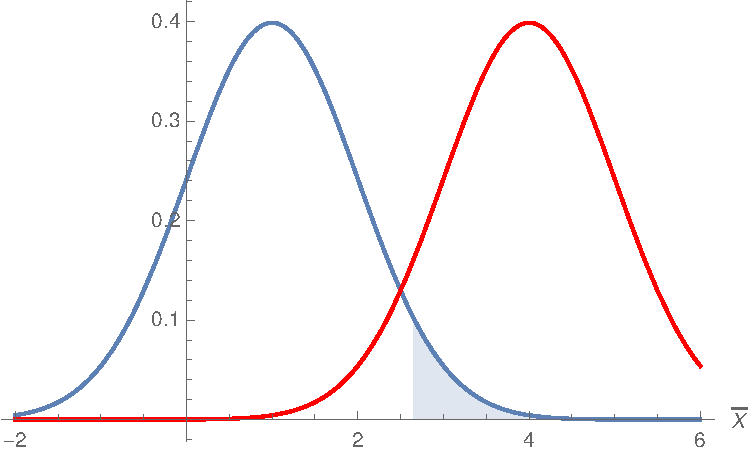
\includegraphics[width=\textwidth]{hypothesis_test.pdf}	
\end{figure}
\end{column}
\begin{column}{0.5\textwidth}
\begin{itemize}
	\item Suppose $\bar{X}$ is normally distributed with $Var\left(\bar{X}\right)=1$ 

	\item We want to test \[
\begin{array}{c}
H_{0}:\qquad\mu_{x}=1\\
H_{1}:\qquad\mu_{x}= 4
\end{array}
\]
	\item The blue and red lines are the PDF of $\bar{x}$ under the null and alternative hypotheses, respectively 

	\item The shaded region is the rejection region with level $\alpha = .05$ that maximizes power. 
	Note that this is for $\bar{X}\ge 2.65$.
	
\end{itemize}

\end{column}

\end{columns}
\end{frame}



\begin{frame}{Rejection Region and Power}
\begin{columns}
\begin{column}{0.5\textwidth}
\begin{figure}	
	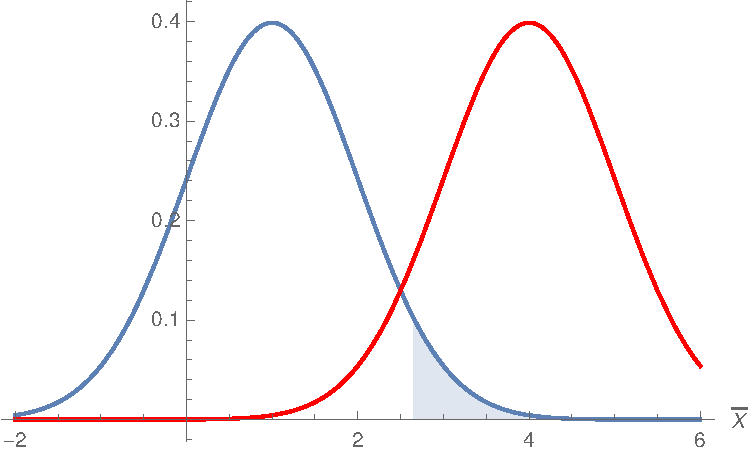
\includegraphics[width=\textwidth]{hypothesis_test.pdf}	
\end{figure}
\end{column}
\begin{column}{0.5\textwidth}
\begin{itemize}
	\item Note that the rejection region is the region where the PDF of
	the alternative hypothesis is high relative to the null hypothesis.
	
	\item The maximum power test with  level $.05$ is the test that rejects for the 5\%
	of the null-hypothesis PDF in which $H_1$'s likelihood (probability density) is highest
	relative to $H_0$'s.

	\item We often take for granted that rejection regions
	are in the tails of the null-hypothesis PDF; this is why.
\end{itemize}

\end{column}

\end{columns}
\end{frame}


\begin{frame}{Review: t Statistics}
\begin{itemize}
	\item Let's return to testing the value of a normally distributed random
	variable's mean, but now let's suppose that $\sigma^2$ is not known (which is
	typically the case).

	\smallskip
	\item Our test statistic instead is\[
		t = \frac{ \overline{X} - a}{n^{-1/2} s}
	\]
	where \[
s=\sqrt{\frac{1}{n-1}\sum_{i=1}^{n}\left(X_{i}-\overline{X}\right)}^2
\]

	\item Here, $t$ has a $t$-distribution with $n-1$ degrees of freedom. 

\end{itemize}
\end{frame}




\begin{frame}{Testing Paradigm}
\begin{itemize}

	\item We focus on different versions of {\bf Wald tests}, which are based on test 
	statistics that are (approximately) normally distributed.

	\medskip
	\item Other paradigms:
	\begin{itemize}
		\item Likelihood Ratio tests and goodness-of-fit-based tests. The idea here is to compare how well
		different models fit the data.

		\item Lagrange multiplier test: for example, testing whether residuals from a restricted model are
		correlated with excluded variables. 
	\end{itemize}
\end{itemize}
\end{frame}


\begin{frame}{Motivating Small Sample $t$-Tests}
\begin{itemize}
	\item Last week we learned that if $N$ is large then,
	\[
		{\bf b}_{OLS} \stackrel{a}{\sim}\mathcal{N}\left(\beta,Var({\bf b}_{OLS})\right)
	\]
	\begin{itemize}
		\item This hinges on knowing $Var({\bf b}_{OLS})$
		\item We rarely know this in practice --- we estimate it instead
		\item Like testing the mean of a normal random variable, estimating the variance
		of the test statistic puts us in a $t$-test situation.
	\end{itemize}
\end{itemize}
\end{frame}

\begin{frame}{$t$-Statistics for OLS Parameters (homoscedasticity)}

\[
\frac{{\bf b}_{OLS,k} - \beta_k}{\sqrt{s^2 \left( {\bf X}' {\bf X}\right)^{-1}_{kk}}} \sim t_{n-K}
\]

\begin{itemize}
	\item where $K$ is the number of parameters,  $s^2$ is the estimator of
	the variance of $\varepsilon$, and \[
	\left( {\bf X}' {\bf X}\right)^{-1}_{kk}
	\]
	refers to the $k$th diagonal element of $\left( {\bf X}' {\bf X}\right)^{-1}$.

	\item Note that the denominator of the above formula is the standard error for the $k$th
	estimated parameter ${\bf b}_{OLS,k} $.

\end{itemize}
\end{frame}


%
%\begin{frame}{The $R^2$ and the Error Variance}
%
%Recall the definition of the $R^2$:
%\[
%	R^2 = \frac{\sum_{i=1}^N (\hat Y_i-\bar Y)^2}{\sum_{i=1}^N(Y_i-\bar Y)^2} = \frac{ESS}{TSS}
%\]
%
%\begin{itemize}
%	\item We call the 	
%\end{itemize}
%
%
%\end{frame}

\begin{frame}{The t-Distribution}

\begin{figure}[htp]
\centering
	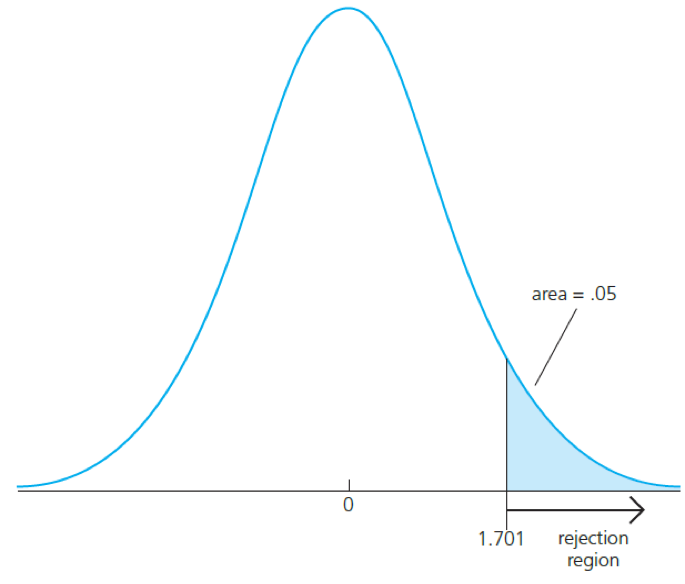
\includegraphics[width=.4\textwidth]{tDistribution}	
\end{figure}

\begin{itemize}
	\item Similar to the $\mathcal{N}(0,1)$ but parametrized by degrees of freedom
	\item The tails are fatter but become $\mathcal{N}(0,1)$ as df go to $\infty$
\end{itemize}
	
\end{frame}

\begin{frame}{Example of Reading a t-Table}
Example of a table of critical values for t distribution from a textbook:
\begin{table}[htp]
\begin{tabular}{ccc}
\hline\hline 
Degrees of Freedom & .10 & .05\\
\hline
1 & 6.31 & 12.71\\
2 & 2.92 & 4.30\\
$\vdots$ & &\\
{\color{red} 28} & 1.70 & {\color{red} \bf 2.05} \\
$\vdots$ & &\\
{\color{red}$\infty$}  & 1.65 & {\color{red} \bf 1.96} \\
\hline
\end{tabular}

\end{table}

\begin{itemize}
	\item If $N$ were very large we would use the $\mathcal{N}(0,1)$ approximation which is exactly the case that $df=\infty$
	\item If $N<\infty$ we can use a table like this, or a computer does it for us
	\item \emph{Example:} If $N=30$, $K=2$, then $df = N-K=28$ the 5\% cutoff value is 2.05 
\end{itemize}

\end{frame}



% HERE

\begin{frame}{An Example (Bivariate Regression)}

\onslide<1->{Suppose I have the following estimated parameters on 30 observations
\begin{align*}
	b_1 =& 1.00\\
	\sum_{i=1}^N(X_i-\bar X)^2 =& 14\\
	\sum_{i=1}^N e_i^2 =& 100
\end{align*}}

\only<2>{
\begin{enumerate}
\item[1.] First, state the hypothesis:
\begin{align*}
	H_0:& \beta_1 = 0\\
	H_1:& \beta_1\ne 0
\end{align*}
\end{enumerate}
}

\only<3>{\begin{enumerate}\item[2.]  Second, calculate $s^2$:
	\begin{align*}
		s^2 =& \frac{1}{N-2}\sum_{i=1}^N( e_i)^2 = 3.45
	\end{align*}
\end{enumerate}
}

\only<4>{\begin{enumerate}\item[3.]  Third, calculate $t$ under $H_0: \beta_1 = 0$:
	\begin{align*}
		t=& \frac{\hat\beta_1 - \beta_1(H_0)}{\sqrt{s^2/\sum_{i=1}^N(X_i-\bar X)^2}} = \frac{1.00}{\sqrt{3.45/14}} = 2.015
	\end{align*} 
	\end{enumerate}
}


\only<5>{\begin{enumerate}\item[4.]  Compare to a critical value
\begin{itemize}
	\item In this case because $df=28$ we DO NOT REJECT the null
	\item Note: $K=2$ assuming we also have a constant term. 
	\item If we had used the $\mathcal{N}(0,1)$ we would narrowly reject the null	
\end{itemize}

	\end{enumerate}
}


\only<6>{\begin{enumerate}\item[5.]  We can also use the critical values to construct a confidence interval
\[
	CI = \hat\beta\pm 2.05\times SE(\hat\beta) = 1.00\pm 2.05\times \sqrt{3.45/14} = [-.017,2.017]
\]
\begin{itemize}
	\item Note that we use the $t$-distribution critical values!
\end{itemize}

	\end{enumerate}
}
\end{frame}



\begin{frame}{Joint hypotheses}
\begin{itemize}
	\item Sometimes we want to test multiple parameters:\[
\begin{array}{c}
H_{0}:\qquad\beta_{exp}=0\quad\text{AND}\quad\beta_{exp2}=0\\
\\
H_{1}:\qquad\beta_{exp}\ne0\quad\text{OR}\quad\beta_{exp2}\ne0
\end{array}
\]

	\item Note that we do not want to do two separate t-tests for this hypothesis. 
\end{itemize}
\end{frame}



\begin{frame}{Illustration of Two t-Tests Failing}

Suppose we have a large sample and t-statistics are $-1$ and $-2$. Do we reject null?

% \only<1>{\vspace{50mm}}

% \only<2>{\vspace{3mm}
\begin{columns}
\begin{column}{0.5\textwidth}
\begin{figure}	
	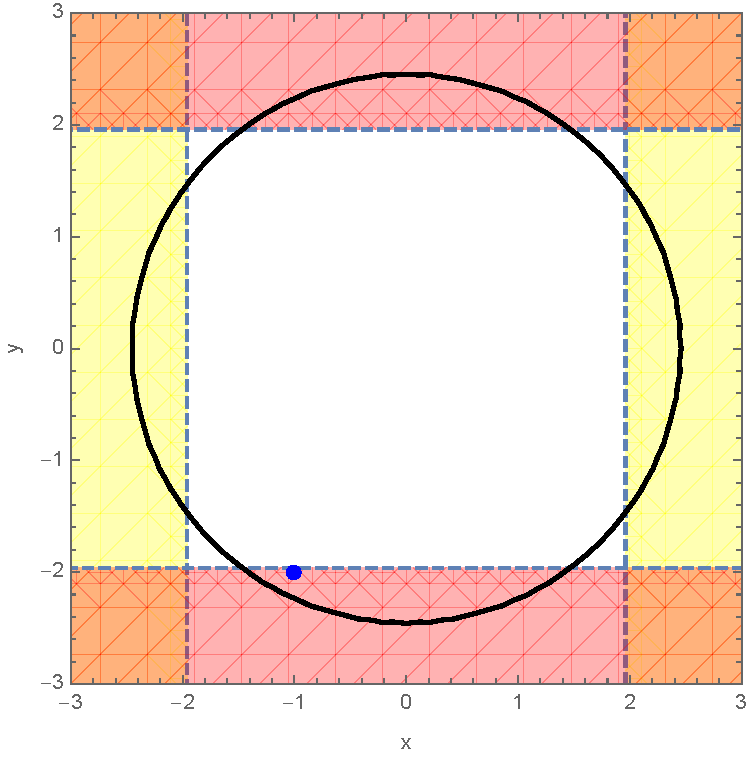
\includegraphics[width=.8\textwidth]{jointTtests1.pdf}	
\end{figure}
\end{column}
\begin{column}{0.5\textwidth}
\small{
If the $t$'s are independent:
\begin{itemize}
	\item The circle contains 95\% of the probability for two independent t-statistics;
	the area outside it is the rejection rejoin for the joint t-test.
	\item The dashed lines are the rejection regions for each of the individual t-tests.  (5\% level)
	\item Even though naively would reject, in actuality \emph{not significant}
	\item What happens with correlated normal RVs?
\end{itemize}
}
\end{column}

\end{columns}

\end{frame}

\begin{frame}{Bivariate normal: independent and correlated}
\begin{columns}
\begin{column}{0.5\textwidth}

	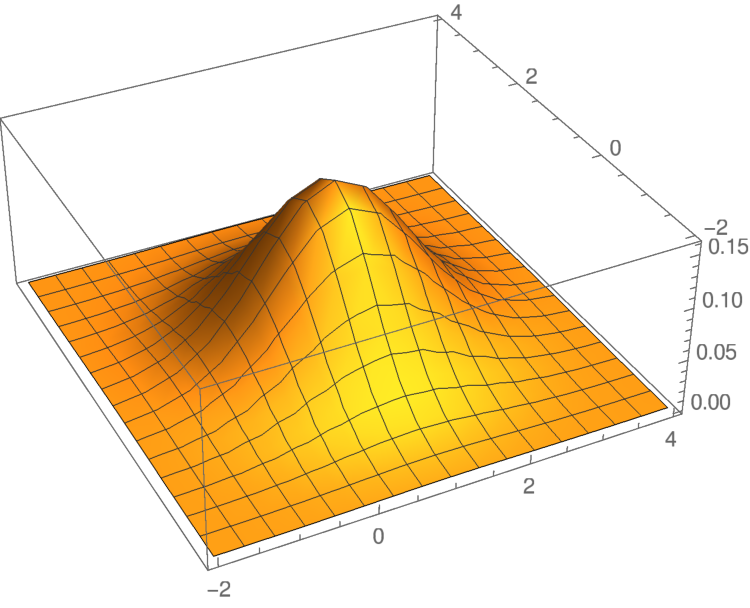
\includegraphics[width=1\textwidth]{joint_normal_ind.pdf}	
\end{column}
\begin{column}{0.5\textwidth}
	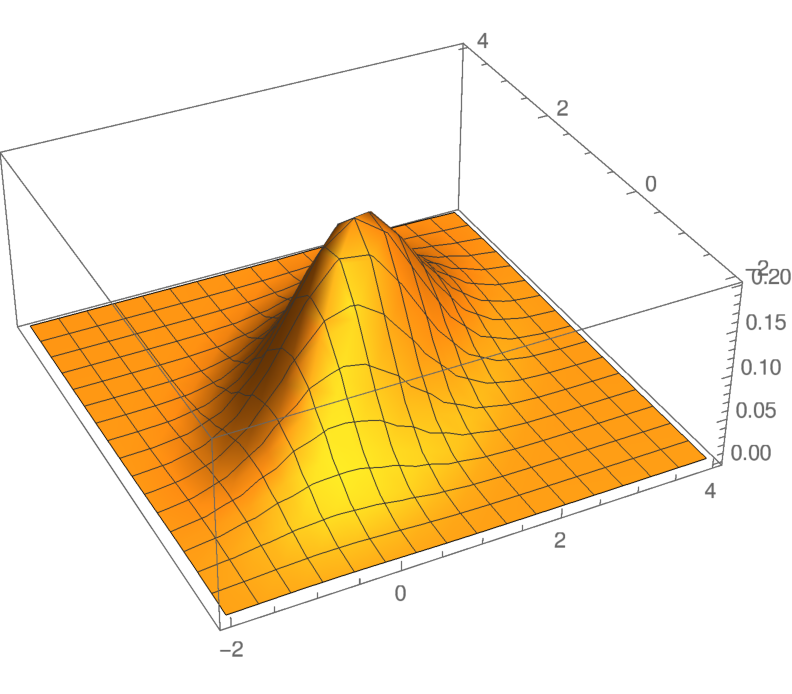
\includegraphics[width=1\textwidth]{joint_normal_corr.pdf}	
\end{column}

\end{columns}
	
\end{frame}


\begin{frame}{T-Tests with correlation}
\vspace{3mm}If the $t$'s are correlated this is the picture:
\begin{columns}
\begin{column}{0.5\textwidth}
\begin{figure}	
	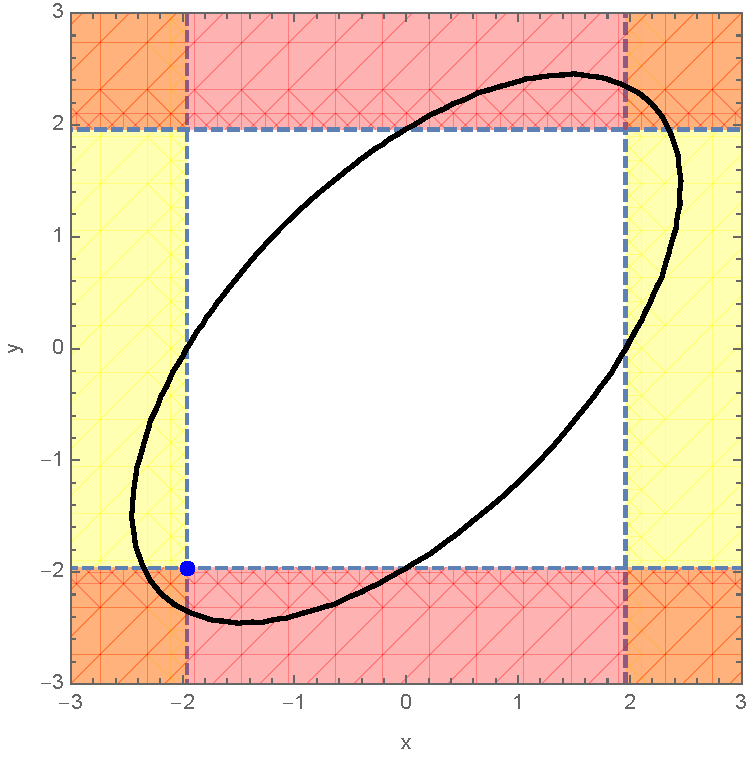
\includegraphics[width=.8\textwidth]{jointTtests2.pdf}	
\end{figure}
\end{column}
\begin{column}{0.5\textwidth}
\begin{itemize}
	\item Now, the area outside the ellipse is the rejection region for the joint t-test (5\% level)
	\item The dashed lines are the rejection regions for each of the individual t-tests.  (5\% level)
	\item Now, notice that even with $t_1 = -2$, $t_2=-2$, which would be a rejection according
	to each of the individual tests, is not a rejection of the joint test. 
\end{itemize}
\end{column}
\end{columns}

\end{frame}




\begin{frame}{Correcting for Correlation: The F-Test}

The issues we have are:
\begin{enumerate}
	\item Testing a joint hypothesis with independent tests will not give the correct type 1 error
	\item Correlated $\hat\beta$'s make things very messy	
\end{enumerate}

 How can we solve this?

\begin{itemize}
	\item First get a statistic that combines both hypotheses
		\begin{itemize}
			\item Should be ``big" when either $t_1$ or $t_2$ or both are big
			\item Should include both $t$'s
		\end{itemize}
	\item Natural candidate:
		\begin{align*}
			F = t_1^2 + t_2^2
		\end{align*}
	\begin{itemize}
		\item Always positive and only big when $t$'s are big
		\item If $t_1$ and $t_2$ are independent normals, then $F\sim \chi^2_2$
		\item If we divide by 2 we have $F_2$ distribution
	\end{itemize}
\end{itemize}	
\end{frame}

\begin{frame}{Correcting for Correlation: The F-Test, Cont'd}
Our candidate test:
	\[
		\frac{1}{2}\times (t_1^2 + t_2^2)
	\]

\begin{itemize}
	\item Has a well understood distribution \emph{when} $t$'s are independent
	\item If not, we can \emph{rotate} the $t$'s so they are
	\begin{itemize}
		\item Non-matrix formula (for 2 parameters):
		\[
			F = \frac{1}{2}\times\frac{t_1^2 + t_2^2 - 2\rho_{t_1,t_2}t_1t_2}{1-\rho_{t_1,t_2}}
		\]
		\item Matrix version (for $k$ parameters):
		\[
			\hat\beta-\beta\sim\mathcal{N}\left(0,\Sigma_{\hat\beta}\right)\Rightarrow \Sigma_{\hat\beta}^{-1/2}\times\left(\hat\beta-\beta\right)\sim\mathcal{N}(0,I)
		\]
		This implies,
		\[
		(\hat\beta-\beta)'\Sigma^{-1}(\hat\beta-\beta)/k\sim\chi^2_k/k = F_k
		\]
		
		
	\end{itemize}	
\end{itemize}	
\end{frame}

\begin{frame}{What is the F Distribution?}
New test statistic:
		\[
			F = \frac{1}{2}\times\frac{t_1^2 + t_2^2 - 2\rho_{t_1,t_2}t_1t_2}{1-\rho_{t_1,t_2}}
		\]

\begin{itemize}
	\item Almost always requires a computer
	\item Ugly formula that follows a simple distribution
	\item In general, for $q$ restrictions, we will calculate the $F$ statistic and it will be distributed $F_q$ ($F_{q,\infty}$ sometimes)
	\item Related to take the sum of squared normal random variables
	\item Critical values will depend on the number of restrictions
	\item Fun fact: for 1 restriction $F = t^2$
\end{itemize}

	
\end{frame}

\begin{frame}{Critical Values of the F}

\begin{figure}
\centering
	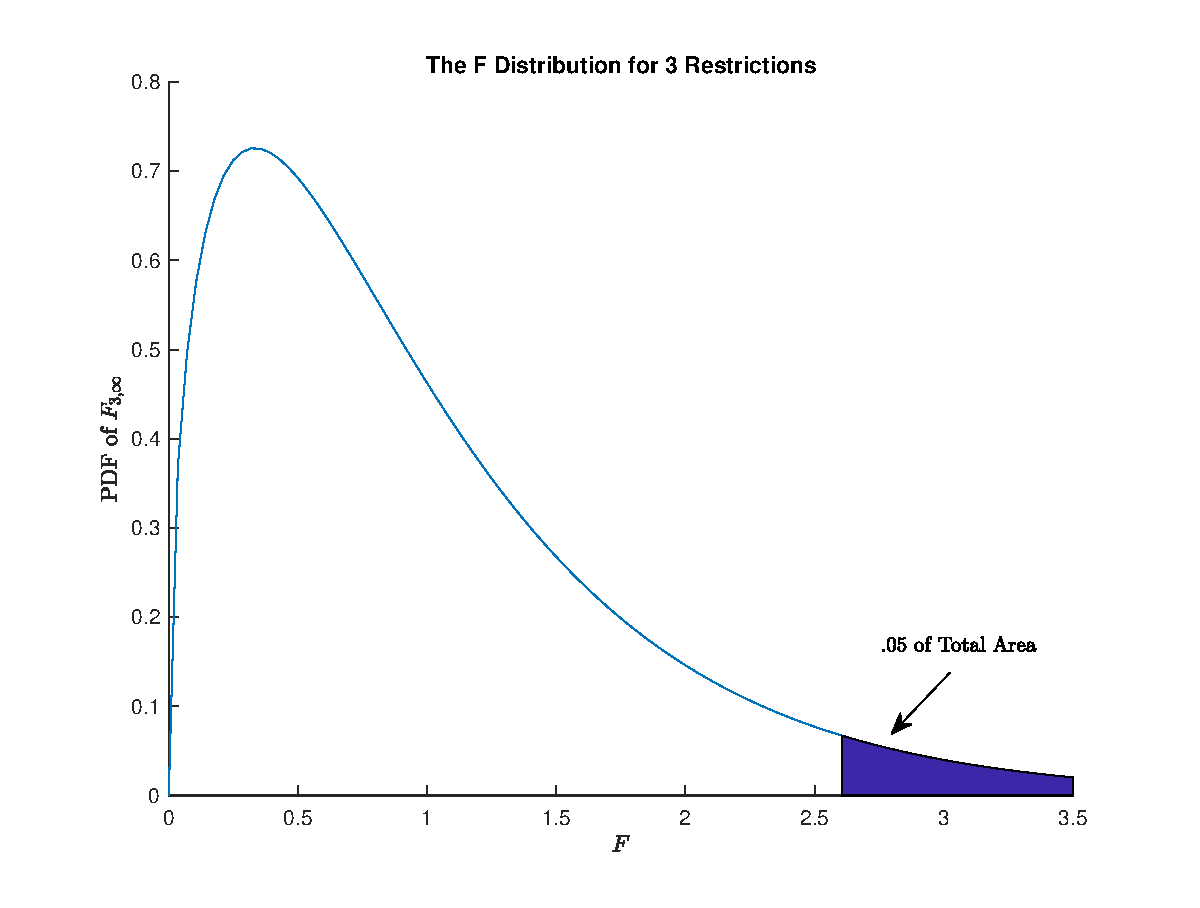
\includegraphics[width=.45\textwidth]{fDistributionk3.eps}	
\end{figure}

\vspace{-5mm}

\begin{itemize}
	\item The distribution looks different than the $t$
	\item But the testing procedure is the same!
	\begin{itemize}
		\item Find a critical value so that $P(F>cv)=.05$
		\item If $F$ is large \emph{given the null} then null is unlikely to be true
		\item Critical value depends on number of restrictions, $q$
	\end{itemize}	
\end{itemize}

\end{frame}




\begin{frame}{F-tests: General Definition}
\begin{itemize}
	\item We are interested in testing the following linear restrictions on the parameters:\[
	{\bf R} \boldsymbol{\beta} = {\bf q}, 
	\]
	where usually $ {\bf q} = {\bf 0}$, but not always.

	\item What would ${\bf R}$ and ${\bf q}$ be if we were testing whether two slopes were equal?

	\item The F statistic (or feasible Wald statistic):\[
F=\frac{\left(\boldsymbol{R}\boldsymbol{b}_{OLS}-\boldsymbol{q}\right)'\left\{ \boldsymbol{R}\left[s^{2}\left(\boldsymbol{X}'\boldsymbol{X}\right)^{-1}\right]\boldsymbol{R}'\right\} ^{-1}\left(\boldsymbol{R}\boldsymbol{b}_{OLS}-\boldsymbol{q}\right)}{J},
\]
which has a $F\left[J,n-K\right]$ distribution, where $J$ is the number of rows of ${\bf R}$ (the number of restrictions).

\end{itemize}
\end{frame}

\begin{frame}{F-tests: equivalent definitions}
\[
F=\frac{\left(\boldsymbol{R}\boldsymbol{b}_{OLS}-\boldsymbol{q}\right)'\left\{ \boldsymbol{R}\left[s^{2}\left(\boldsymbol{X}'\boldsymbol{X}\right)^{-1}\right]\boldsymbol{R}'\right\} ^{-1}\left(\boldsymbol{R}\boldsymbol{b}_{OLS}-\boldsymbol{q}\right)}{J},
\]
\begin{itemize}
	\item We could also write:\[
		F = \frac{SSE_{CLS} - SSE_{OLS}}{Js^2},
	\]
	where $SSE_{OLS}$ is the sum of squared residuals for the (unrestricted) OLS estimator, $SSE_{CLS}$
	is the sum of squared residuals under the {\bf constrained least squares} estimator with constraints ${\bf R} \boldsymbol{\beta} = {\bf q}$.

	\item We are not going to delve into constrained least squares, but the point here is that there are two equivalent ways to think about
	the F-statistic: (1) as a Wald statistic, which is based on comparing an asymptotically normal parameter estimate to a hypothesized value, 
	and (2) as an assessment of how much better the unconstrained model fits than the constrained model. 
\end{itemize}
\end{frame}




\begin{frame}{Non-Nested Models}
\begin{itemize}
	\item We have considered only nested models thus far. When testing \[
	{\bf R} \boldsymbol{\beta} = {\bf q}, 
	\]
	we are testing a restricted linear model against alternative hypothesis of 
	an unrestricted linear model, \emph{ which includes the restricted model as a special
	case}.

	\medskip
	\item Sometimes we want to compare non-nested models, which brings us to
	model selection. The main idea
	is to balance the model's goodness of fit and number of parameters: see
	adjusted $R^2$, {\bf Akaike Information Criterion}, {\bf Bayesian
	Information Criterion}. Machine learning approaches typically
	try to compare models by directly assessing out-of-sample performance.
	 More on this stuff later and/or next semester.

\end{itemize}
\end{frame}


\begin{frame}{OLS standard errors}
\begin{itemize}
	\item A useful identity for linear algebra:
\begin{align*}
\operatorname { Var } (a \mathbf{Z} ) = a^2 \operatorname { Var }(\mathbf{Z})\\
\operatorname { Var } (A \mathbf{Z} ) = A \operatorname { Var }(\mathbf{Z}) A'
\end{align*}

\smallskip
\item Since ${\bf b}_{OLS} = ({\bf X} '{\bf X} )^{-1} {\bf X} '{\bf y}$,
\[
\operatorname { Var } ({\bf b}_{OLS} | {\bf X}) = ({\bf X} '{\bf X} )^{-1} {\bf X}' \operatorname { Var } ({\bf y} | {\bf X})  {\bf X}  ({\bf X} '{\bf X} )^{-1}
\]

\smallskip
\item Recalling that $\operatorname { Var } ( \mathbf{y} |\mathbf{X} )  = \operatorname { Var } ( \mathbf{\varepsilon} | \mathbf { X } ) $,
\[
\operatorname { Var } ({\bf b}_{OLS} | {\bf X}) = ({\bf X} '{\bf X} )^{-1} {\bf X}' \operatorname { Var } ( \mathbf{\varepsilon} | \mathbf { X } )  {\bf X}  ({\bf X} '{\bf X} )^{-1}
\]
\end{itemize}
\end{frame}


\begin{frame}{OLS standard errors}
\[
\operatorname { Var } ({\bf b}_{OLS} | {\bf X}) = ({\bf X} '{\bf X} )^{-1} {\bf X}' \operatorname { Var } ( \mathbf{\varepsilon} | \mathbf { X } )  {\bf X}  ({\bf X} '{\bf X} )^{-1}
\]
\begin{itemize}

\smallskip
\item With homoscedasticity, $\operatorname { Var } ( \mathbf{\varepsilon} | \mathbf { X } ) = \sigma^2 {\bf I}$, and
this simplifies to \[
\operatorname { Var } ({\bf b}_{OLS} | {\bf X}) =  \sigma^2 ({\bf X} '{\bf X} )^{-1} 
\]

\smallskip
\item Without homoscedasticity, we can still use the ``sandwich'' formula above. 
\end{itemize}
\end{frame}



\begin{frame}{Example: Engel Curves}
\begin{itemize}
	\item Engel curves refer to the relationship between a household's expenditure share on a 
	good and income (or total expenditure).

	\item Engel curves for food are typically downward sloping -- as total expenditure of a household
	increases, the proportion of its expenditure dedicated to food falls.
	\begin{itemize}
		\item Expenditure on food still rises as total expenditure rises, but less than proportionally,
		so that food's expenditure \emph{share} falls.
	\end{itemize}
\end{itemize}
\end{frame}



\begin{frame}{Food Engel Curves}
\begin{columns}
\begin{column}{0.5\textwidth}
	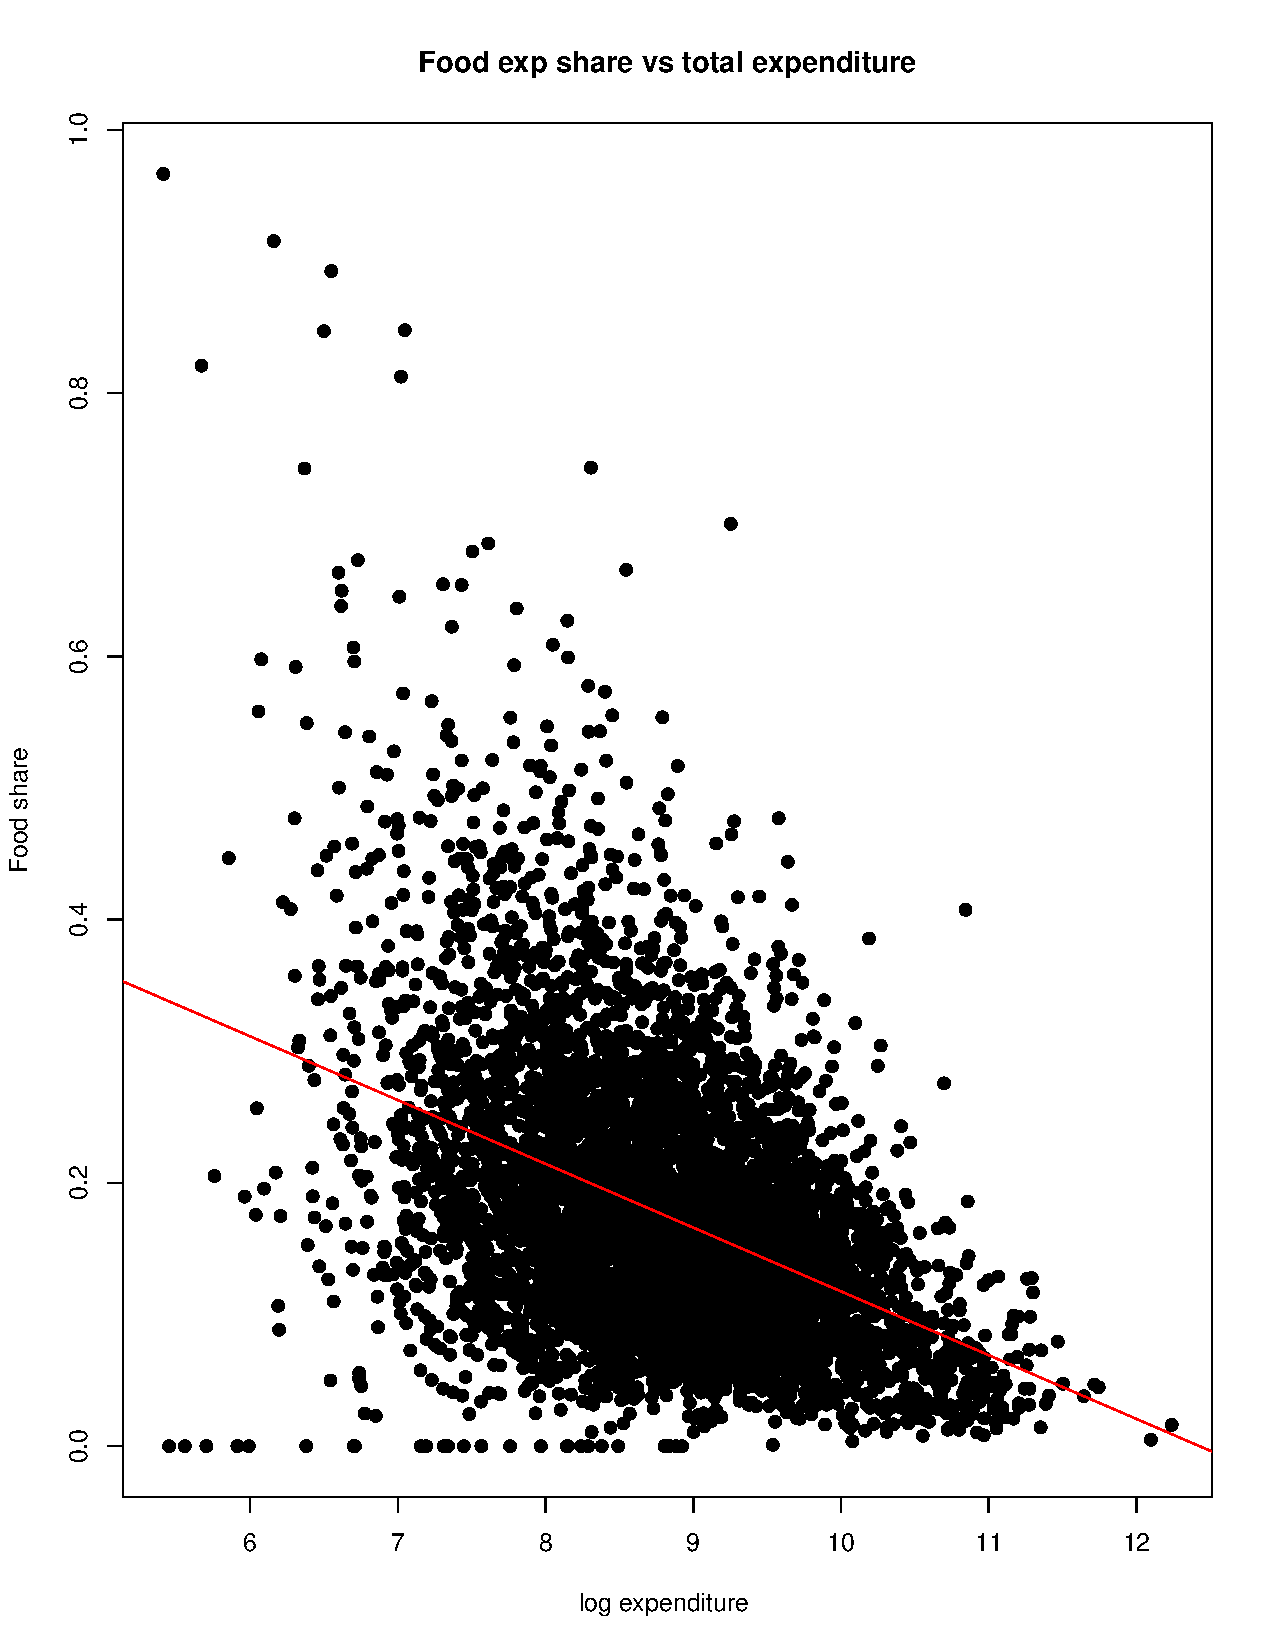
\includegraphics[width=.7\textwidth]{engle1.pdf}	

{\tiny Data source: BLS Consumer Expenditure Survey data}

\end{column}
\begin{column}{0.5\textwidth}
\begin{itemize}
	\item If we plotted total food expenditure (rather than the expenditure share), the heteroscedasticity would go in the other direction.
\end{itemize}
\end{column}
\end{columns}
\end{frame}





\begin{frame}{Heteroscedasticity Robust Standard Errors I}
\begin{itemize}
	\item It is common to compute Eicker-Huber-White standard errors, which 
	is a different estimator of $\boldsymbol{\Sigma}$ that is consistent
	even if each observation has a different variance $\sigma_i^{2}$:\[
\left(\boldsymbol{X}'\boldsymbol{X}\right)^{-1}\left(\boldsymbol{X}'\text{diag}\left(e_{1}^{2},e_{2}^{2},\dots,e_{n}^{2}\right)\boldsymbol{X}\right)\left(\boldsymbol{X}'\boldsymbol{X}\right)^{-1}
\]

	\item Statistical software typically makes it easy to use this estimator for
	 $\boldsymbol{\Sigma}$ instead of the standard homoscedastic estimator.

	\item Heteroscedasticity-robust standard errors still perform well even if homoscedasticity
		holds, so there's little reason to even assume homoscedasticity when computing standard errors. 
\end{itemize}
\end{frame}





\begin{frame}{Heteroscedasticity Robust Standard Errors II}
\begin{itemize}
	\item We can rewrite the {\bf heteroscedasticity-consistent} (or {\bf heteroscedasticity-robust}) standard error estimator as:\[
n^{-1}\left(n^{-1}\boldsymbol{X}'\boldsymbol{X}\right)^{-1}\left(n^{-1}\boldsymbol{X}'\text{diag}\left(e_{1}^{2},e_{2}^{2},\dots,e_{n}^{2}\right)\boldsymbol{X}\right)\left(n^{-1}\boldsymbol{X}'\boldsymbol{X}\right)^{-1},
\]
where the middle piece of this ``sandwich'' estimator can be written as\[
	n^{-1} \sum_{i} {\bf x}_i {\bf x}'_i  e_i^2
	\]

	\item Notice that this is the sample analog of $V\left[{\bf x}_i \varepsilon_i \right]$. What's going on with the robust
	standard error formula is we're constructing an estimate of \[
		n^{-1} E\left[{\bf x}_i {\bf x}'_i\right]^{-1} V\left[{\bf x}_i \varepsilon_i \right] E\left[{\bf x}_i {\bf x}'_i\right]^{-1}.
	\]
	This is known as a sandwich estimator of variance. 
\end{itemize}
\end{frame}





\begin{frame}[fragile]\frametitle{Doing a Heteroscedastic F-Test in \texttt{R}}
	Let us revisit the wage equation:
	\[
		\log(Wage_i) = \beta_0 + \beta_1 Age_i + \beta_2 Age_i^2 + \beta_3 Educ_i + \varepsilon_i
	\]
	
	\begin{itemize}{\small 
		\item New question: does experience/age matter at all?
		\item New hypothesis:
			\begin{align*}
				H_0&: \beta_1 = 0\text{ and } \beta_2=0\\
				H_a&: \beta_1 \ne 0\text{ or } \beta_2\ne 0
			\end{align*}
		\item How do we test in \texttt{R} using heteroscedastic robust standard errors?}
	\end{itemize}

\vspace{5mm}

% We need a new command:
% \begin{itemize}{\small 
% 	\item First, we need the \verb!car! package
% 	\begin{itemize}{\footnotesize
% 		\item As a reminder, to install packages use the command: \verb!install.packages("car")!
% 		\item As a reminder, to load a package use the command: \verb!library(car)! }
% 	\end{itemize}
% }
% \end{itemize}
\end{frame}





\begin{frame}[fragile]\frametitle{Doing a Heteroscedastic F-Test in \texttt{R}, Cont'd}
	Let us revisit the wage equation:
	\[
		\log(Wage_i) = \beta_0 + \beta_1 Age_i + \beta_2 Age_i^2 + \beta_3 Educ_i + \varepsilon_i
	\]
\begin{columns}
\begin{column}{0.45\textwidth}
\vspace{-14mm}
\begin{figure}[htp]
\flushleft
	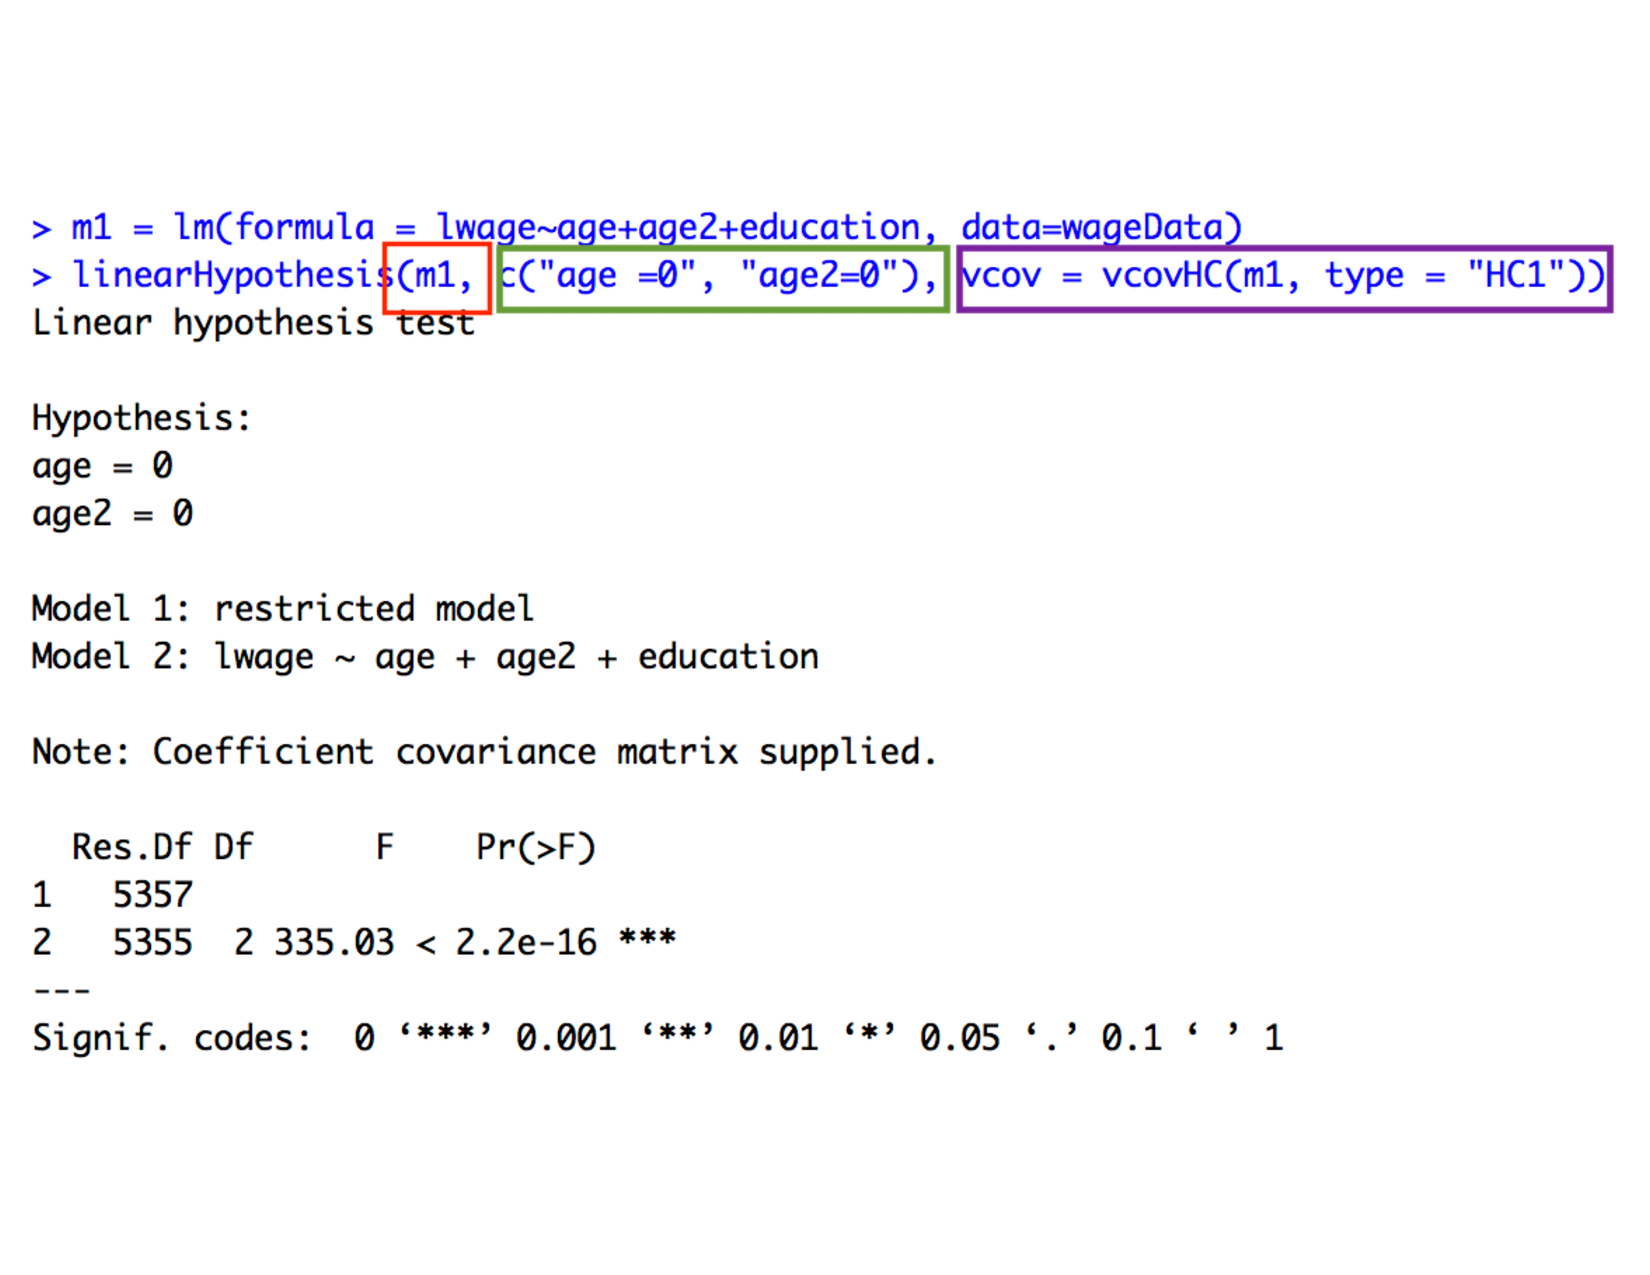
\includegraphics[width = 1.05\textwidth]{testingMultipleRestrictionsExample.pdf}	
\end{figure}

\end{column}
\begin{column}{0.55\textwidth}
\begin{itemize}{\footnotesize
	\item {\bf \color{red} Red} box is the name of the model
	\item {\bf \color{green} Green} box is the list of hypotheses:
				\begin{itemize}{\scriptsize 
					\item List enclosed by the \texttt{c()} command
					\item Each restriction is enclosed in quotes, one equal sign and uses the names of the variables from the model
					\item Don't forget to separate commands with commas}
				\end{itemize}
				
	\item {\bf \color{purple} Purple} box is the variance-covariance argument}
\end{itemize}

\end{column}

\end{columns}
\vspace{3mm}
{\scriptsize
Command without boxes:
% \begin{verbatim}
% 	linearHypothesis(m1, c("age =0", "age2=0"), vcov = vcovHC(m1, type = "HC1"))	
% \end{verbatim}
}
	
\end{frame}




\begin{frame}{Outliers}
\begin{itemize}
	\item {\bf Outliers} refer to observations that are ``far away'' from the rest of the data. 
	They can be due to errors in the data.  There is no standard formal definition. 

	\medskip
	\item What to do? Greene:``\emph{It is difficult to draw firm general conclusions... It remains likely that in very
	small samples, some caution and close scrutiny of the data are called for.}'' I'd say that's true even in large samples,
	but there isn't a generally accepted way of quantifying what counts as appropriate ``caution and close scrutiny.''


\end{itemize}
\end{frame}


\begin{frame}{Removing Outliers?}
\begin{itemize}
\item Removing extreme outliers (in $x$) from datasets is often considered good practice. But we should be mindful
		about why as dropping observations creates the potential for manipulation. 

	\medskip
	\item Sometimes extreme outliers are just errors, in which case they should almost certainly be dropped.

	\medskip
	\item Even if they aren't errors, they may reflect a different mode in the data generating process. They may require
		a different or more general model to account for them properly. Consider the justificaiton of a linear
		model based on Taylor's theorem (local linear approximation). With such a justification for your modeling
		strategy, it would not make sense to include an outlier in $x$.
	\medskip
	\item It's important to be transparent about how dropped outliers affect results. 

\end{itemize}
\end{frame}




\begin{frame}{Outliers and Leverage}
\begin{itemize}
\item One way to find influential observations is to calculate the {\bf leverage} of each observation $i$. We begin with the hat matrix:
\begin{align*}
P = {\bf X} ({\bf X} '{\bf X})^{-1}  {\bf X}'
\end{align*}
and consider the diagonal elements, which are labeled $h_{ii}$
\begin{align*}
h_{ii} = \bf{x}_i `({\bf X} '{\bf X})^{-1}  \bf{x}_i
\end{align*}

\medskip
\item This tells us how influential an observation is in our estimate of ${\bf b}_{OLS}$.\\
Particularly important for $\{0,1\}$ dummy variables with uneven groups.
\end{itemize}
\end{frame}



\begin{frame}{Leave One Out Regression}
\begin{itemize}
\item This is sometimes called the {\bf Jackknife}
\item Sometimes it is helpful to know what would happen if we omitted a single observation $i$
\item Turns out we don't need to run $N$ regressions
\begin{align*}
{\bf b}_{-i} &= ({\bf X}_{-i}'{\bf X}_{-i})^{-1} {\bf X}_{-i}' {\bf y}_{-i} \\
&={\bf b}_{OLS} -  ({\bf X} '{\bf X})^{-1} {\bf x}_i  \tilde{e}_i  \quad \mbox{ where } \tilde{e}_i = (1-h_{ii})^{-1} e_i
\end{align*}
\item $\tilde{e}_i $ has the interpretation of the LOO prediction error.
\item high leverage observations move ${\bf b}_{OLS}$ a lot.
\end{itemize}
\end{frame}

%\begin{frame}[fragile]{Leverage and QQ plots}
%\begin{lstlisting}
%library(car)
%fit <- lm(mpg~disp+hp+wt+drat, data=mtcars)

%# Assessing Outliers
%outlierTest(fit) # Bonferonni p-value for most extreme obs
%qqPlot(fit, main="QQ Plot") #qq plot for studentized resid 
%leveragePlots(fit) # leverage plots
%\end{lstlisting}
%\end{frame}

%\begin{frame}{Leverage Plot}
%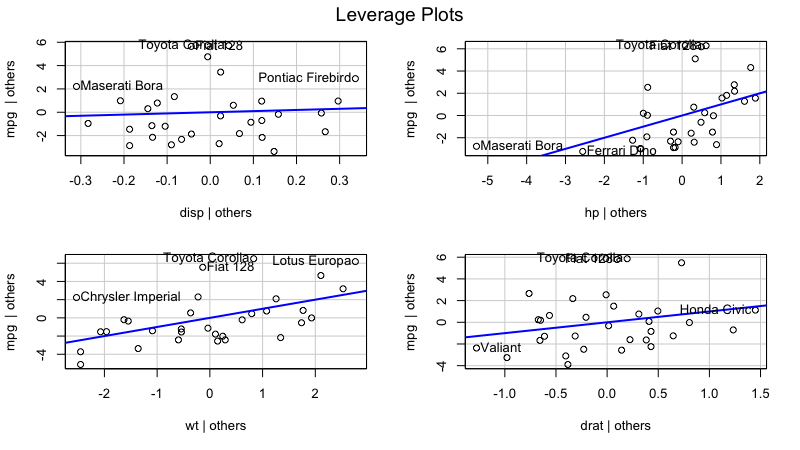
\includegraphics[scale=.45]{leverage_plot.png}
%\end{frame}




\begin{frame}{Heteroskedasticity Consistent (HC) Variance Estimates}
What we need is a consistent estimator for $e^2_i$.
\begin{align*}
\mathbf{V}_{OLS}^{HC0}&= ({\bf X}' {\bf X})^{-1} \left(\sum_{i=1}^N {\bf x}_i {\bf x}_i'  e_i^2 \right) ({\bf X}' {\bf X})^{-1} \\
\mathbf{V}_{OLS}^{HC1}&= ({\bf X}' {\bf X})^{-1} \left(\sum_{i=1}^N {\bf x}_i {\bf x}_i'  e_i^2 \right) ({\bf X}' {\bf X})^{-1} \cdot \left(\frac{n}{n-k}  \right)
\end{align*}
Could use $\tilde{e}_i$ instead of $e_i$ for a better estimate
\begin{align*}
\mathbf{V}_{OLS}^{HC2}&= ({\bf X}' {\bf X})^{-1} \left(\sum_{i=1}^N (1-h_{ii})^{-1} {\bf x}_i {\bf x}_i' e_i^2 \right) ({\bf X}' {\bf X})^{-1} \\
\mathbf{V}_{OLS}^{HC3}&= ({\bf X}' {\bf X})^{-1} \left(\sum_{i=1}^N (1-h_{ii})^{-2} {\bf x}_i {\bf x}_i' e_i^2 \right) ({\bf X}' {\bf X})^{-1} \\
\end{align*}
\end{frame}


\begin{frame}{Heteroskedasticity Consistent (HC) Variance Estimates}
\begin{itemize}
\item We know that $\mathbf{V}_{OLS}^{HC3} > \mathbf{V}_{OLS}^{HC2} > \mathbf{V}_{OLS}^{HC0}$ because $(1- h_{ii}) <1$.
\item \texttt{Stata} uses $HC1$ as the default and it is what most people refer to when they say {\bf robust standard errors}.
	These are the Eicher-Huber-White SE's.
\item Note: failure to correct for heteroscedasticity can lead to size distortions (a rate of type I errors that differs from what you intend). 
\item $HC3$ are the most conservative and also place the most weight on potential outliers.
\end{itemize}
\end{frame}


\begin{frame}[fragile]{Heteroskedasticity Consistent (HC) Variance Estimates}
\footnotesize
\begin{lstlisting}
dat <- data.frame(X = matrix(rnorm(2000*5), 2000), y = rnorm(2000))
res<-feols(y~X..[1:5], dat)
se(res,"iid")
se(res,"hc1")
\end{lstlisting}
To read about SE implementation:
\url{ https://declaredesign.org/r/estimatr/articles/mathematical-notes.html}
\end{frame}




\begin{frame}{Heteroscedasticity vs. Correlation}
\begin{itemize}
	\item Recall that we defined the homoscedasticity assumption as:\[
	Var\left(\boldsymbol{\varepsilon} \right) =\sigma^2 {\bf I}
	\]
	this assumption has two aspects:
	\begin{enumerate}
		\item The disturbance for each observation has the same variance
		\item Imposing zero correlation between disturbances for different observations
	\end{enumerate}

	\item The terminology can be misleading here, because what people refer to as ``heteroscedasticity-robust''
	standard errors (the variance estimators on the previous slide) are robust to violations of 1 but not 2. 

	\item We need to do a bit more to estimate standard errors in a way that is robust to correlated data. 

\end{itemize}
\end{frame}


\begin{frame}{Correlation I}
\begin{itemize}
	\item The baseline assumptions of the linear regression framework imply that
	the disturbances are uncorrelated across observations.  There are many ways for this to be violated. 
	\begin{itemize}
		\item Example 1: we might have county-level data for a regression and be concerned
		that different counties within a given state have correlated disturbances because
		all counties are subject to the same (unobserved) state-level policies.
		\item Example 2: time series data (asset prices), and we are worried that some unobserved
		factors within the disturbances are serially correlated
		\item Example 3: county level data again, and we are worried about geographically
		correlated factors such as weather. 
	\end{itemize}
\end{itemize}
\end{frame}


\begin{frame}{Correlation II}
 Different correlation patterns call for different estimators of $\boldsymbol{\Sigma}$, the variance of ${\bf b}_{OLS}$
	Some common alternatives to the no-correlation baseline:
\begin{enumerate}
	\item Clustered standard errors, when there is correlation between observations
	within well-defined groups, but no correlation between observations in different groups. 
	\item Newey-West standard errors (and extensions) to deal with serial correlation
	in time series data.
	\item Conley-Newey-West standard errors that allow for correlation in multiple dimensions
	(especially popular in the context of spatially explicit models).
\end{enumerate}
\end{frame}


\begin{frame}{Clustering I}
\begin{itemize}
	\item Suppose data are organized into distinct groups $g=1,2,\dots,G$. Let $g\left(i\right)$
	be the group identity of observation $i$. 
	\begin{itemize}
		\item e.g., with county-level data, we have $g\left(Manhattan\right)=NY$.
	\end{itemize}


	\medskip
	\item We assume $E\left[\varepsilon_i \varepsilon_j\right]=0$ as long as $g\left(i\right)\ne g\left(j\right)$,
	and we do not restrict the correlation $E\left[\varepsilon_i \varepsilon_j\right]$
	for observations within the same group.

	\medskip
	\item Intuition: the linear regression framework with no correlation in observations will overstate
	the precision of our estimates. If we add another observation within a cluster, and that observation
	is highly correlated with the other observations, it's not actually as good as adding another independent observation. 
\end{itemize}
\end{frame}

\begin{frame}{Clustering II}
\begin{itemize}
	\item Recall the sandwich formula for standard errors:\[
		n^{-1} E\left[{\bf x}_i {\bf x}'_i\right]^{-1} V\left[{\bf x}_i \varepsilon_i \right] E\left[{\bf x}_i {\bf x}'_i\right]^{-1}.
	\]

	\item The estimator for the middle part without clustering was\[
	{\bf V}\left[{\bf x}_i \varepsilon_i \right] = n^{-1} \sum_{i} {\bf x}_i {\bf x}'_i  e_i^2
	\]

	\item With clustering, it will be \[
	{\bf V}_{clu} = n^{-1} \sum_{i=1}^{n}\sum_{j=1}^{n} {\bf x}_i {\bf x}'_j e_i e_j {\bf I}\left[g\left(i\right)==g\left(j\right)\right]
	\]
	where the ${\bf I}$ function is 1 when $i,j$ come from the same group and zero otherwise.

\end{itemize}
\end{frame}


\begin{frame}{Clustering III}
\begin{itemize}
	\item The cluster-robust estimate of standard errors will be consistent as the number of groups 
	gets large.

	\item Note that this estimator adds extra terms (covariance terms) to the estimate of variance,
	so this is going to make standard errors larger as long as covariances $E\left[\varepsilon_i \varepsilon_j\right]$ are positive. 

	\item Thus, if standard formulas are used in the presence of cluster-correlated disturbances, 
	standard errors will be too small.

	\item Statistical software packages typically make it easy to compute cluster-robust errors.
	
	\item Clustering often makes a {\bf huge} difference in standard errors.

\end{itemize}
\end{frame}

\begin{frame}{Correlation III}

 Consider the cluster-robust estimator of the ``meat'' part of the sandwich estimator: \[
	{\bf V}_{clu} = n^{-1} \sum_{i=1}^{n}\sum_{j=1}^{n} {\bf x}_i {\bf x}'_j  e_i e_j {\bf I}\left[g\left(i\right)==g\left(j\right)\right]
	\]

\medskip
 For Conley-Newey-West standard errors (where there is correlation between ``nearby'' observations),
	procedure is similar.

\medskip
	 The difference is that instead of the 1/0 indicator function for ${\bf I}$, we will have a 
	weighting (or kernel) function which takes on values $\approx 1$ for ``nearby'' observations and goes to zero for
	observations that are far apart.


\end{frame}



\begin{frame}{Clustered SE's}
\begin{align*}
\widehat { \boldsymbol { V } } _ { OLS } ^ { \mathrm { CR } 1 } = \left( \boldsymbol { X } ^ { \prime } \boldsymbol { X } \right) ^ { - 1 } \left( \sum _ { g = 1 } ^ { G } \boldsymbol { X } _ { g } ^ { \prime } \boldsymbol { e }_ { g }  \boldsymbol { e }_ { g } ^ { \prime } \boldsymbol { X } _ { g } \right) \left( \boldsymbol { X } ^ { \prime } \boldsymbol { X } \right) ^ { - 1 }\\
\widehat { \boldsymbol { V } } _ { OLS } ^ { \mathrm { CR } 3 } = \left( \boldsymbol { X } ^ { \prime } \boldsymbol { X } \right) ^ { - 1 } \left( \sum _ { g = 1 } ^ { G } \boldsymbol { X } _ { g } ^ { \prime } \widetilde { \boldsymbol { e } } _ { g }  \widetilde { \boldsymbol { e } } _ { g } ^ { \prime } \boldsymbol { X } _ { g } \right) \left( \boldsymbol { X } ^ { \prime } \boldsymbol { X } \right) ^ { - 1 }
\end{align*}
\begin{itemize}
\item Can replace  $\mathbf{e}_g  \rightarrow \tilde { \mathbf{e}}_g $ for leave-one out like $HC3$ (these are called $CR3$).
\end{itemize}
\end{frame}


\begin{frame}[fragile]{Clustering in R}
\begin{lstlisting}
feols(y~ x1 + x2, data=df, vcov=~group_id )
feols(y~ x1 + x2, data=df, vcov=~group_id+time_id)
\end{lstlisting}
\end{frame}





%\begin{frame}{Delta Method}
%\begin{itemize}
%	\item
%\end{itemize}
%\end{frame}




\begin{frame}{Bootstrap I}
\begin{itemize}
	\item Another approach to estimating the standard errors of ${\bf b}_{OLS}$
	is the {\bf bootstrap}

	\item The basic idea:
	\begin{enumerate}
		\item Simulate a new data set (same number of observations) by sampling (with replacement) from the original data set

		\item Estimate ${\bf b}_{OLS,s}$ for the new data set.

		\item Repeat lots of times, resulting in a bunch of different estimates of ${\bf b}_{OLS,s}$, say $s=1,\dots,10000$

		\item Look at the variance of the ${\bf b}_{OLS,s}$ estimates 
		across the various simulated data sets. This is your estimate of $\boldsymbol{\Sigma}$, or $Var\left({\bf b}_{OLS}\right)$
	\end{enumerate}

\end{itemize}
\end{frame}


\begin{frame}{Bootstrap II}
\begin{itemize}
	\item The bootstrap's main appeal is that it can provide a better finite-sample
	approximation of the distribution of the parameter estimates.
	\begin{itemize}
		\item Note that the Eicker-Huber-White standard errors estimates are \emph{consistent}, but
		not generally \emph{unbiased} in finite samples
		\item The bootstrap is probably worth trying if you're ever working with
		 non-linear estimators (which can be consistent but are typically not unbiased in finite samples). 
	\end{itemize}

	\medskip
	\item Also, it can potentially deliver good estimates of standard errors even with 
	correlated errors, but this depends on the version of the bootstrap (see {\bf block bootstrap}).
	 Exploring formally the  conditions under which the bootstrap works well is beyond our scope. 
\end{itemize}
\end{frame}




%\begin{frame}{Confidence Intervals}
%\begin{itemize}
%	\item
%\end{itemize}
%\end{frame}



\begin{frame}{Confidence Intervals I}
\begin{itemize}
	\item Note that if 	\[
		{\bf b} \sim\mathcal{N}\left(\boldsymbol{\beta},\Sigma)\right),
	\]
	then \[
		b_{k} \sim\mathcal{N}\left(\beta_k,\Sigma_{kk}\right),	
	\]
	and \[
	Pr\left[ b_{k} - z_{\left(1-\alpha/2\right)} \sqrt{\Sigma_{kk}} \le \beta_k \le b_k +  z_{\left(1-\alpha/2\right)}  \sqrt{\Sigma_{kk}}  \right] =\alpha 
	\]
	where $ z_{\left(1-\alpha/2\right)} $ is the value such that the CDF of the standard normal distribution is $1-\alpha/2$. 	

\end{itemize}
\end{frame}




\begin{frame}{Confidence Intervals II}
\begin{itemize}
	\item Similarly, when \[
		\frac{b_k - \beta_k}{\sqrt{\hat{\Sigma}_{kk}}} \sim t_{n-K}
	\]
	because the variance $\Sigma_{kk}$ has to be estimated, then
 \[
	\hspace*{-1cm} Pr\left[ b_{k} - t_{\left(1-\alpha/2\right),n-K} \sqrt{\hat{\Sigma}_{kk}} \le \beta_k \le b_k +  t_{\left(1-\alpha/2\right),n-K}  \sqrt{\hat{\Sigma}_{kk}}  \right] =\alpha 
	\]
	where $ t_{\left(1-\alpha/2\right),n-K} $ is the value such that the CDF of the t-distribution with $n-K$ degrees of freedom is $1-\alpha/2$. 	

\end{itemize}
\end{frame}



\begin{frame}{Confidence Intervals III}
\begin{itemize}
	\item We define the $1-\alpha$ {\bf confidence interval} for $b_{k}$ as \[
	\left(b_{k} - t_{\left(1-\alpha/2\right),n-K} \sqrt{\hat{\Sigma}_{kk}} , b_k +  t_{\left(1-\alpha/2\right),n-K}  \sqrt{\hat{\Sigma}_{kk}} \right)
	\]

	\smallskip
	\item Note that this confidence interval is a function of the data -- the end points of the confidence interval 
	are statistics and therefore random variables in their own right. 

	\smallskip
	\item Defining the confidence interval in this way, the probability that the confidence interval contains
	the true parameter is $1-\alpha$ (if the asymptotic distribution of the estimator is taken as the true distribution). 
	That is, if $\alpha=.05$, this is called a 95\% confidence interval, and there
	is a 95\% chance it will contain the true parameter (assuming that the asymptotic approximation holds). 

\end{itemize}
\end{frame}

\begin{frame}{Summary}
\begin{itemize}
	\item Linear regression theory gives us formulas for estimating $Var\left({\bf b}_{OLS}\right)$

	\item We can use that variance estimator to test hypotheses about parameters (using t-Tests
	and f-Tests) as well as construct confidence intervals. 

	\item When the baseline assumptions of the linear regression model are violated (due to
	correlation or heteroscedasticity), we need to use somewhat more complex formulas
	to estimate  $Var\left({\bf b}_{OLS}\right)$.

\end{itemize}
\end{frame}



\end{document}